%% ==========================================================================
%%  Two-Run Maze Solver (ATmega32A) -- Line-by-Line Explanation and
%%  Algorithmic Audit
%%
%%  Build:  pdflatex maze_solver_audit.tex   (run twice for the ToC)
%%  Source analysed: branch maze-solver, directory code/main.
%%  Method: static reading of the source only. Nothing was simulated or
%%  executed to produce the analysis.
%% ==========================================================================
\documentclass[11pt,a4paper]{article}

\usepackage[T1]{fontenc}
\usepackage[utf8]{inputenc}
\usepackage{lmodern}
\usepackage[margin=2.3cm]{geometry}
\usepackage{microtype}
\usepackage{amsmath,amssymb,amsthm}
\usepackage{booktabs,tabularx,longtable,array}
\usepackage{enumitem}
\usepackage[dvipsnames]{xcolor}
\usepackage{listings}
\usepackage{tikz}
\usetikzlibrary{arrows.meta,positioning}
\usepackage{caption}
\usepackage[hidelinks]{hyperref}

\setlength{\emergencystretch}{3em}
\setlist{itemsep=2pt,topsep=4pt}

%% identifiers with underscores, printed verbatim in typewriter
\newcommand{\code}[1]{\texttt{\detokenize{#1}}}
\newcommand{\file}[1]{\textsf{\detokenize{#1}}}
\newcommand{\bigO}[1]{\mathcal{O}\!\left(#1\right)}

\theoremstyle{plain}
\newtheorem{lemma}{Lemma}
\newtheorem{theorem}{Theorem}
\newtheorem{corollary}{Corollary}
\theoremstyle{definition}
\newtheorem{definition}{Definition}
\newtheorem{finding}{Finding}

\definecolor{codebg}{RGB}{248,248,248}
\definecolor{codekw}{RGB}{0,70,140}
\definecolor{codecm}{RGB}{90,110,90}
\lstset{
  language=C,
  basicstyle=\ttfamily\footnotesize,
  keywordstyle=\color{codekw}\bfseries,
  commentstyle=\color{codecm}\itshape,
  backgroundcolor=\color{codebg},
  frame=single, rulecolor=\color{black!25},
  numbers=left, numberstyle=\tiny\color{black!50}, numbersep=6pt,
  breaklines=true, columns=fullflexible, keepspaces=true,
  showstringspaces=false, tabsize=4,
  morekeywords={uint8_t,uint16_t,uint32_t,int16_t,int32_t,size_t,wm_play_t,
                turn_dir_t,turn_result_t,sonar_t,sonar_id_t,gyro_xyz_t}
}

\title{\textbf{Two-Run Maze Solver on the ATmega32A}\\[4pt]
\large Line-by-Line Explanation and Algorithmic Audit}
\author{Code audit of branch \texttt{maze-solver}, directory \file{code/main}}
\date{28 September 2026}

\begin{document}
\maketitle

\begin{abstract}
\noindent
This document explains and audits the firmware of a two-run maze-solving
robot built on an ATmega32A with three HC-SR04 ultrasonic rangers, an
MPU-6050 gyroscope and an L298N motor driver. Run~1 explores the maze with
a strict left-hand wall-following rule and logs one byte per decision
point. Between the runs the log is collapsed by a string-rewriting rule
that removes every dead-end excursion. Run~2 replays the collapsed route,
checking each junction against a stored signature before acting on it.
The algorithm is a \emph{depth-first traversal with physical backtracking}
followed by \emph{stack reduction} of the traversal. No grid, adjacency
matrix, frontier queue or visited set exists anywhere in the code, and
the document explains why. Each module is analysed for what it does, how
it does it and why it was built that way. The reduction is proved correct
for loop-free mazes, the time and space costs are derived, the edge cases
are catalogued, and a prioritised list of findings and optimisations is
given.
\end{abstract}

\tableofcontents
\newpage

%% ==========================================================================
\section{Scope and method}
%% ==========================================================================

\paragraph{What was analysed.} Every source file in \file{code/main} of
branch \texttt{maze-solver} at commit \texttt{8037520} (5\,093 lines of C
including headers). The standalone bench images in \file{code/motor_test}
and \file{code/driver_check} are hardware diagnostics and are outside the
scope of the algorithm audit.

\paragraph{How.} Static reading of the source. Nothing was simulated or run
to produce this analysis: every claim about behaviour follows from the code
as written, and every complexity bound is derived analytically. Line numbers
quoted as \file{file.c:N} refer to that commit.

\paragraph{Files and roles.}

\begin{center}
\small
\begin{tabularx}{\linewidth}{@{}l r X@{}}
\toprule
File & Lines & Role \\
\midrule
\file{wallmem.h/.c}   & 155+321 & Junction log: record format, left-hand rule, collapse, replay, EEPROM persistence \\
\file{solver.h/.c}    & 46+708  & Top-level finite-state machine for both runs \\
\file{sonar.h/.c}     & 56+304  & Round-robin ultrasonic ranging, filtering, openness, front voting \\
\file{drive.h/.c}     & 51+416  & Straight-line wall-centring controller, emergencies, wall recovery \\
\file{turn.h/.c}      & 85+423  & Gyro-closed 90\textdegree{} and 180\textdegree{} pivots, back-off pulses \\
\file{heading.h/.c}   & 54+157  & Gyro bias calibration, heading integration, rocking detection \\
\file{mpu6050.h/.c}, \file{i2c.h/.c} & 25+123, 22+128 & Gyro driver on a bounded, self-recovering I\textsuperscript{2}C bus \\
\file{main.c}         & 162     & Boot order and the fixed-rate control loop \\
\file{timer, panel, power, resetlog, debug, telemetry, motors} & 978 & Time base, button/LED, supply monitor, reset forensics, serial log, CSV telemetry, PWM \\
\file{config.h}       & 879     & Every tunable constant, with measured justifications \\
\bottomrule
\end{tabularx}
\end{center}

%% ==========================================================================
\section{High-level overview}
%% ==========================================================================

\subsection{The problem as the robot sees it}

The maze is built from 40\,cm cells (\code{CORRIDOR_WIDTH_CM}). The robot
has \emph{no wheel encoders}, so it cannot measure distance travelled except
as \emph{time} $\times$ \emph{estimated speed} (\code{TRAVEL_SPEED_CMS}).
It can do two things reliably:
\begin{enumerate}
  \item \textbf{Classify the cell it is standing in} from three range
        readings (left, front, right) as a 3-bit openness vector $(F,L,R)$.
  \item \textbf{Rotate by a known relative angle} (90\textdegree{} or
        180\textdegree) using an integrated gyro rate.
\end{enumerate}
It cannot tell \emph{where} it is in absolute coordinates. Every design
decision in the solver follows from that constraint.

\subsection{Paradigm}

The firmware combines three algorithmic stages:

\begin{enumerate}
  \item \textbf{Online depth-first traversal (run 1).} The left-hand rule
        (\code{WallMem_LeftHand}, \file{wallmem.h:108}) chooses, at every
        decision point, the first open direction in the fixed rotational
        order \textsc{Left} $\succ$ \textsc{Forward} $\succ$ \textsc{Right}
        $\succ$ \textsc{U-turn}. On a maze without loops this is exactly a
        \emph{depth-first search} of the maze tree in which the child order
        is fixed by geometry and \emph{backtracking is a physical U-turn} at
        a dead end.
  \item \textbf{Offline path reduction (between runs).} The log of turns is
        collapsed by repeatedly rewriting any triple $(A,\,U,\,B)$ into the
        single net turn $(A+B+2) \bmod 4$ (\code{WallMem_Reduce},
        \file{wallmem.c:62}). This removes every excursion into a dead end
        and leaves the turns of the start-to-exit path. It is the
        run-length analogue of popping a DFS stack on backtrack.
  \item \textbf{Guarded replay (run 2).} The reduced string is consumed one
        record per decision point, and each record's stored signature must
        equal the openness vector observed now (\code{WallMem_Play},
        \file{wallmem.c:107}). A mismatch degrades to the memory-free
        left-hand rule.
\end{enumerate}

\begin{center}
\small
\begin{tabularx}{\linewidth}{@{}l l X@{}}
\toprule
Candidate paradigm & Used? & Where / why not \\
\midrule
DFS            & \textbf{Yes} (implicit) & Left-hand rule = DFS with fixed child order and physical backtracking \\
Stack reduction & \textbf{Yes} & \code{WallMem_Reduce} removes backtracked subtrees \\
BFS            & No & Needs to expand many frontier cells ``at once''; a robot can only be in one place, and a BFS executed physically costs $\Theta(V^2)$ travel in the worst case \\
Dijkstra / A*  & No & Need a map with coordinates and edge lengths; there is no odometry to build one \\
Flood fill (micromouse) & No & Needs the robot's $(x,y)$ cell index at all times; time $\times$ speed drifts without bound and is never corrected (\file{wallmem.h:24}) \\
\bottomrule
\end{tabularx}
\end{center}

\subsection{Data structures}

There is \textbf{no grid matrix, adjacency list or node class}. The maze
graph is \emph{implicit}: it exists only in the physical world and is
discovered one decision point at a time. The single algorithmic data
structure is a byte array used as a traversal log:

\begin{lstlisting}[firstnumber=21]
static uint8_t s_log[WALLMEM_MAX_RECORDS];
static uint8_t s_count      = 0;
static uint8_t s_overflow   = 0;
static uint8_t s_play_index = 0;
static uint8_t s_solved     = 0;
\end{lstlisting}

Each record is one byte (\file{wallmem.h:30--47}):

\begin{center}
\small
\begin{tabular}{@{}c|c|c|c|c|c|c|c@{}}
bit 7 & bit 6 & bit 5 & bit 4 & bit 3 & bit 2 & bit 1 & bit 0\\\hline
0 & $F$ open & $L$ open & $R$ open & 0 & 0 & \multicolumn{2}{c}{turn (2 bits)}
\end{tabular}
\end{center}

\begin{itemize}
  \item \textbf{Signature} (bits 6--4): the raw openness the sonars reported
        on arrival. Stored raw rather than as a junction enum so that run 2
        compares like with like.
  \item \textbf{Turn} (bits 1--0): quarter-turns \emph{clockwise},
        $F{=}0,\;R{=}1,\;U{=}2,\;L{=}3$. This encoding makes rotation
        composition addition in $\mathbb{Z}_4$, which is what turns the
        collapse rule into one line of arithmetic.
  \item \textbf{Zero bits} (7, 3, 2; mask \code{0x8C}): a structural
        checksum. Erased EEPROM reads \code{0xFF}, which fails the mask, so a
        blank or half-written cell can never parse as a record.
\end{itemize}

The EEPROM image (\file{wallmem.c:126--141}) is an 8-byte header plus the
records:

\begin{center}
\small
\begin{tabular}{@{}l l l@{}}
\toprule
Offset & Content & Note \\
\midrule
+0, +1 & magic \texttt{'W'}, \texttt{'M'} & +0 cleared first, written \emph{last} (commit byte) \\
+2 & format version (1) & \\
+3 & record count $n$ & rejected if $n > 48$ \\
+4 & flags (bit 0 = solved) & \\
+5 & CRC-8 (poly \code{0x07}, init \code{0xFF}) & over +2..+4 and all records \\
+6, +7 & reserved & \\
+8 \ldots & $n$ record bytes & \\
\bottomrule
\end{tabular}
\end{center}

\subsection{Why not a grid search?}

A grid algorithm needs a cell index $(r,c)$ for every sensor reading.
Without encoders, the index would come from integrating
$\hat v\,\Delta t$ with $\hat v$ an estimate that the logs show varying from
34 to 43\,cm/s between runs. The index error grows linearly in travelled
distance and nothing ever resets it, so after a few cells the map would
disagree with reality. The chosen design depends only on two quantities
whose errors do \emph{not} accumulate across cells: the local openness
vector (re-measured at every junction) and relative rotation (re-zeroed at
every stop). That is the main design rationale of the whole codebase.

%% ==========================================================================
\section{System architecture and execution model}
%% ==========================================================================

\subsection{Boot sequence (\textsf{main.c:27--105})}

\begin{enumerate}
  \item \code{Motors_Init(); Motors_Stop();} \emph{first}. A reset leaves
        the L298N inputs floating, and the last commanded motion can persist,
        so the motors are stopped before anything else can fail.
  \item \code{Panel_Init()} claims the LED pin and arms the button pull-up.
  \item UART, 1\,ms timer, I\textsuperscript{2}C, sonar pins and ADC are
        initialised, then interrupts are enabled (\code{sei}).
  \item \code{ResetLog_Report()} prints why the chip last reset, from
        \code{MCUCSR} plus variables kept in \code{.noinit} SRAM.
  \item \code{MPU6050_Init()} and \code{Gyro_CalibrateFull()} (500 samples,
        spread-checked).
  \item \code{Solver_Init()} loads a saved route if one validates, then
        \code{Solver_Begin()} arms the robot (nothing moves before a button
        press).
  \item \code{wdt_enable(WDTO_250MS)} and the control loop.
\end{enumerate}

\subsection{The control loop (\textsf{main.c:107--161})}

Condensed from \file{main.c:107--161}. The loop runs one \emph{tick} every \code{CONTROL_TICK_MS} $= 20$\,ms:

\begin{lstlisting}[numbers=none]
for (;;) {
    wdt_reset();
    if ((int32_t)(millis() - next_tick) < 0) continue;  /* wait for tick */
    next_tick += CONTROL_TICK_MS;
    tick_start = millis();
    if ((int32_t)(millis() - next_tick) > (int32_t)(CONTROL_TICK_MS * 3))
        next_tick = millis() + CONTROL_TICK_MS;         /* re-base, no burst */
    MPU6050_ReadAll(&g);          /* 1: gyro (X, Y, Z in one burst)     */
    Motion_Update(&g);            /* 2: rocking detector                 */
    Heading_Add(g.z, CONTROL_TICK_MS);  /* 3: integrate yaw             */
    Sonar_Task();                 /* 4: exactly one ping, round-robin    */
    Power_Task();                 /* 5: supply rail sample               */
    Panel_Task();                 /* 6: button debounce, LED blink       */
    /* ... fill tick_ctx_t ... */
    Solver_Tick(&ctx);            /* 7: behaviour                        */
    if ((millis() - tick_start) > TICK_OVERRUN_WARN_MS) overruns++;
    Telemetry_Tick(&ctx);         /* 8: CSV, after the deadline check    */
}
\end{lstlisting}

\textbf{Why this shape.}
\begin{itemize}
  \item \emph{Fixed rate.} The gyro is integrated as rate $\times$ \code{dt}
        with a constant \code{dt}. The PD gains in the drive controller are
        tuned per tick. Both are only valid if the tick really is constant,
        so overruns are counted and reported.
  \item \emph{Re-base instead of catch-up.} After a long blocking operation
        (a pivot), firing the missed ticks back-to-back would feed the
        controller several samples with near-zero spacing. The loop skips
        them instead.
  \item \emph{Sensing before behaviour, telemetry after the deadline.} The
        solver sees a consistent snapshot of the tick. Printing is excluded
        from the timing measurement, so turning up the trace cannot itself
        cause overruns.
  \item \emph{Watchdog.} Fed once per pass and inside every blocking wait.
        A hang reboots the chip within 250\,ms, and the first thing
        \code{main} does is stop the motors.
\end{itemize}

Pivots, braking and calibration are \emph{blocking} sub-loops with their
own 5\,ms gyro schedule (\code{TURN_TICK_MS}). The main tick is suspended
while they run, and they feed the watchdog themselves.

%% ==========================================================================
\section{Component analysis}
%% ==========================================================================

\subsection{Wall-follower memory (\textsf{wallmem.h}, \textsf{wallmem.c})}

\subsubsection{Record helpers (\textsf{wallmem.h:83--113})}

Condensed (comments removed, one-liners joined):


\begin{lstlisting}[numbers=none]
static inline uint8_t WallMem_Turn(uint8_t rec) { return rec & WM_TURN_MASK; }
static inline uint8_t WallMem_Sig (uint8_t rec) { return rec & WM_SIG_MASK;  }
static inline uint8_t WallMem_RecordIsSane(uint8_t rec)
    { return (rec & WM_ZERO_MASK) ? 0u : 1u; }
static inline uint8_t WallMem_PackSig(uint8_t f, uint8_t l, uint8_t r)
    { return (f ? WM_OPEN_F : 0) | (l ? WM_OPEN_L : 0) | (r ? WM_OPEN_R : 0); }
static inline uint8_t WallMem_IsDecision(uint8_t f, uint8_t l, uint8_t r)
    { return (f && !l && !r) ? 0u : 1u; }
static inline uint8_t WallMem_LeftHand(uint8_t f, uint8_t l, uint8_t r) {
    if (l) return WM_TURN_L;
    if (f) return WM_TURN_F;
    if (r) return WM_TURN_R;
    return WM_TURN_U;
}
\end{lstlisting}

\begin{itemize}
  \item \code{WallMem_IsDecision}: \textbf{what} --- a cell is a decision
        point unless it is a plain corridor (front open, both sides walled).
        \textbf{Why} --- corridor cells carry no information and are not
        logged. The \emph{same} predicate gates recording in run 1 and
        consumption in run 2, so the two runs cannot fall out of step: run 2
        can only consume a record where run 1 could have written one. Note
        that corners (\textsc{Forced\_Left}/\textsc{Forced\_Right}) and dead
        ends \emph{are} decision points. This matters for the collapse
        (Lemma~\ref{lem:fold}).
  \item \code{WallMem_LeftHand}: the whole exploration policy in four lines.
        It is also the fallback policy for a failed replay, because it needs
        no memory at all.
\end{itemize}

\subsubsection{Recording (\textsf{wallmem.c:40--48})}

\begin{lstlisting}[firstnumber=40]
uint8_t WallMem_Record(uint8_t f_open, uint8_t l_open, uint8_t r_open, uint8_t turn) {
    if (s_count >= WALLMEM_MAX_RECORDS) { s_overflow = 1; return 0; }
    // Assembling the byte by OR-ing two masked fields is the only place a
    // record is built, so the invariant "bits 7,3,2 are zero" holds by
    // construction rather than by everyone remembering it.
    s_log[s_count++] = (uint8_t)(WallMem_PackSig(f_open, l_open, r_open) |
                                 (turn & WM_TURN_MASK));
    return 1;
}
\end{lstlisting}

\begin{itemize}
  \item Line 41: bounds check \emph{before} the write. On overflow the record
        is dropped, a sticky flag is set, and the caller reports it. A
        truncated log would replay into a wall, so overflow later
        disqualifies the run from being saved (\file{solver.c:645}).
  \item Line 45: this is the only place a record is assembled. Both OR-ed
        operands are masked, so the zero bits (7, 3, 2) are clear by
        construction.
\end{itemize}

\subsubsection{Collapse (\textsf{wallmem.c:62--93}), line by line}

\begin{lstlisting}[firstnumber=62]
uint8_t WallMem_Reduce(uint8_t *stray_u_out) {
    uint8_t i, folded, stray = 0;

    do {
        folded = 0;
        for (i = 1; (uint8_t)(i + 1) < s_count; i++) {
            if (WallMem_Turn(s_log[i]) == WM_TURN_U) {
                uint8_t a   = WallMem_Turn(s_log[i - 1]);
                uint8_t b   = WallMem_Turn(s_log[i + 1]);
                uint8_t net = (uint8_t)((a + b + 2u) & WM_TURN_MASK);

                s_log[i - 1] = (uint8_t)(WallMem_Sig(s_log[i - 1]) | net);
                memmove(&s_log[i], &s_log[i + 2],
                        (size_t)(s_count - (uint8_t)(i + 2)));
                s_count = (uint8_t)(s_count - 2);
                folded = 1;
                break;                      // indices moved; rescan
            }
        }
    } while (folded);

    // A U-turn that survives has no pair of neighbours to fold into: it sits at
    // one end of the string, or the maze has a loop so the walk never came back
    // the way it went in. Either way the remaining string is not a route.
    for (i = 0; i < s_count; i++) {
        if (WallMem_Turn(s_log[i]) == WM_TURN_U) stray++;
    }
    if (stray_u_out) *stray_u_out = stray;
    if (stray == 0) s_solved = 1;
    s_play_index = 0;
    return s_count;
}
\end{lstlisting}

\begin{description}[style=nextline]
  \item[Lines 65--81 (outer \code{do}/\code{while})] Repeat until a full
        scan finds nothing to fold. A fold can \emph{create} a new U
        (e.g.\ $L,U,R \mapsto U$), so a single pass is not enough.
  \item[Line 67 (scan bounds)] $i$ starts at 1 and stops while $i+1<n$, so
        the U at index $i$ always has both neighbours $i-1$ and $i+1$. For
        $n<3$ the body never runs. The cast to \code{uint8_t} keeps the
        comparison in the same width as \code{s_count}.
  \item[Lines 69--71 (fold arithmetic)] Excursion $=$ turn $A$, drive, turn
        $U$, drive back, turn $B$. Headings compose additively in quarter
        turns, so the net rotation is $A+2+B \pmod 4$. \code{& 3} is the
        modulo.
  \item[Line 73 (keep $A$'s signature)] The surviving record describes the
        junction as it looked on \emph{first arrival}, which is exactly how
        run 2 will arrive there.
  \item[Lines 74--76 (delete two records)] \code{memmove} shifts the tail
        left by two. The length $n-(i+2)\ge 0$ because $i+1<n$.
        \code{memmove} (not \code{memcpy}) is required because source and
        destination overlap.
  \item[Line 78 (\code{break})] Indices have moved, so the scan restarts
        from the beginning. This keeps the code short, and it is the source
        of the quadratic cost analysed in \S\ref{sec:complexity}.
  \item[Lines 86--90 (stray check)] Any U that survives has no neighbour
        pair to fold into. The route is only marked solved if none remain.
\end{description}

\subsubsection{Replay (\textsf{wallmem.c:107--121})}

\begin{lstlisting}[firstnumber=107]
wm_play_t WallMem_Play(uint8_t f_open, uint8_t l_open, uint8_t r_open,
                       uint8_t *turn_out) {
    uint8_t rec, seen;

    if (s_play_index >= s_count) return WM_PLAY_EXHAUSTED;

    rec  = s_log[s_play_index];
    seen = WallMem_PackSig(f_open, l_open, r_open);

    if (WallMem_Sig(rec) != seen) return WM_PLAY_MISMATCH;

    s_play_index++;
    if (turn_out) *turn_out = WallMem_Turn(rec);
    return WM_PLAY_OK;
}
\end{lstlisting}

\textbf{Why the signature check comes first.} If a pivot overshot and the
robot is in the wrong corridor, the next junction will almost certainly
look different from the stored one. Checking \emph{before} consuming the
record converts a silent navigation error into a detected fault. The cursor
is advanced only on a match.

\subsubsection{Persistence (\textsf{wallmem.c:163--240})}

\begin{itemize}
  \item \code{crc8}: bitwise CRC-8, polynomial $x^8+x^2+x+1$ (\code{0x07}),
        8 shift steps per byte. The table-free form costs no flash table and
        runs only at save/load time.
  \item \code{WallMem_Save}: the magic byte at $+0$ is \emph{invalidated
        first} and \emph{written last}. A brown-out anywhere in between
        leaves no magic, so the next boot rejects the block and explores
        again instead of driving half a route. The records are read back and
        compared. \code{eeprom_update_byte} skips unchanged cells, which
        saves EEPROM wear.
  \item \code{WallMem_Load}: rejects on magic, version, $n>48$, any record
        failing the zero-bit mask, or a CRC mismatch. The records are staged
        in a local \code{tmp[48]} and copied into \code{s_log} only after
        every check passes, so a bad block never overwrites a good log.
\end{itemize}

\subsection{Solver state machine (\textsf{solver.c})}

\subsubsection{State and bookkeeping}

\code{wm_state_t} (\file{solver.c:47}) has twelve states (full transition
table in \S\ref{sec:fsm}). The bookkeeping variables:
\begin{itemize}
  \item \code{s_open_l}, \code{s_open_r}, \code{s_block_f},
        \code{s_deadend}: consecutive-tick counters (debounce, saturating at
        255).
  \item \code{s_passing}: ``already decided \textsc{Forward} here''. It
        suppresses re-logging the same junction on every tick while driving
        through it.
  \item \code{s_post_turn}, \code{s_moving_since}, \code{s_wall_seen_l/r},
        \code{s_approach_ms}: set up the approach length for an opening that
        continues straight on from the cell the robot pivoted in (below).
  \item \code{s_exploring} (run 1 vs.\ run 2), \code{s_degraded} (replay
        abandoned), \code{s_pending_turn}, \code{s_uturn_dir}.
\end{itemize}

\subsubsection{Debounce and openness (\textsf{solver.c:105--140})}

Condensed:


\begin{lstlisting}[numbers=none]
static void update_debounce(void) {
    if (Sonar_HasSample(SONAR_LEFT) && Sonar_IsOpen(SONAR_LEFT))
         { if (s_open_l < 255) s_open_l++; } else s_open_l = 0;
    if (Sonar_HasSample(SONAR_RIGHT) && Sonar_IsOpen(SONAR_RIGHT))
         { if (s_open_r < 255) s_open_r++; } else s_open_r = 0;
    if (Sonar_FrontBlocked()) { if (s_block_f < 255) s_block_f++; } else s_block_f = 0;
    if (Sonar_HasSample(SONAR_LEFT)  && !Sonar_IsOpen(SONAR_LEFT))  s_wall_seen_l = 1;
    if (Sonar_HasSample(SONAR_RIGHT) && !Sonar_IsOpen(SONAR_RIGHT)) s_wall_seen_r = 1;
    if (Sonar_FrontBlocked() && !Sonar_IsOpen(SONAR_LEFT) && !Sonar_IsOpen(SONAR_RIGHT))
         { if (s_deadend < 255) s_deadend++; } else s_deadend = 0;
}
static void read_openness(uint8_t *f, uint8_t *l, uint8_t *r) {
    *l = (s_open_l  >= OPENING_CONFIRM) ? 1 : 0;
    *r = (s_open_r  >= OPENING_CONFIRM) ? 1 : 0;
    *f = (s_block_f >= OPENING_CONFIRM) ? 0 : 1;
}
\end{lstlisting}

\begin{itemize}
  \item \textbf{What}: each side is ``open'' only after
        \code{OPENING_CONFIRM} $=2$ consecutive ticks say so. A dead end
        needs \code{DEADEND_CONFIRM} $=3$.
  \item \textbf{Why \code{Sonar_HasSample}}: after a flush a side holds the
        \code{SONAR_NO_ECHO} placeholder, which reads as open. Without this
        guard an unmeasured side could be confirmed as an opening in the
        start cell.
  \item \textbf{Why the counters saturate at 255}: an \code{uint8_t} that
        wrapped to 0 after 256 ticks would briefly look like ``not open''.
  \item \textbf{Why the dead-end threshold is higher}: a false U-turn is the
        most expensive error. It costs two pivots and writes a U into the log.
\end{itemize}

\subsubsection{Decision (\textsf{solver.c:166--215})}

\code{decide_turn(f,l,r)}: in run 1, or after a replay failure, it applies
\code{WallMem_LeftHand} and (run 1 only) records the decision. In run 2 it
calls \code{WallMem_Play}. On \code{MISMATCH} or \code{EXHAUSTED} it prints
the stored and observed junction types and then, by default, sets
\code{s_degraded} and returns the left-hand answer for the rest of the run.
(With \code{WALLMEM_HALT_ON_MISMATCH} set it halts instead.) The rationale
is that a stale instruction is worse than no instruction, and the
left-hand rule still reaches the exit of a loop-free maze from any
position.

\subsubsection{\texttt{pick\_180\_dir} (\textsf{solver.c:146})}

A dead-end U-turn rotates towards the side with more clearance. An
in-place pivot is asymmetric: the front corners sweep about 17\,cm into the
side being turned towards, the rear corners only about 11\,cm the other
way. It requires a margin of \code{UTURN_DECIDE_MARGIN_CM} before
preferring a side, and falls back to \code{UTURN_TIE_DIR}. This is called in
\code{WM_RECAL} \emph{before} \code{Sonar_Flush}, because the flush destroys
the readings it depends on.

\subsubsection{Per-tick guards (\textsf{solver.c:310--348})}

Before the state switch, two global checks run every tick:
\begin{enumerate}
  \item \textbf{Run limit}: in DRIVING through RECOVER, more than
        \code{MAX_RUN_MS} (5\,min) since the button press $\Rightarrow$
        stop and \code{WM_FAULT}. It is counted per run, not since boot, so
        waiting armed between runs never trips it.
  \item \textbf{Gyro lost}: in STARTUP through RECOVER, \code{!MPU6050_Healthy()} (reads failing for
        \code{GYRO_FAIL_MS} $=100$\,ms) $\Rightarrow$ stop and
        \code{WM_FAULT}. Without a gyro every turn and all straight-line
        damping would be meaningless.
\end{enumerate}

\subsubsection{The states}

\begin{description}[style=nextline]
  \item[\code{WM_ARMED} (350)] Motors off. Prints the integrated heading
        every 2\,s, so the gyro scale can be calibrated by turning the robot
        by hand. A long press erases the saved route and re-arms for run 1.
        A short press enters \code{WM_STARTUP}.
  \item[\code{WM_STARTUP} (385)] Waits \code{STARTUP_DELAY_MS} (3\,s) for
        hands to leave the chassis. Then: quick gyro recalibration,
        heading reset, sonar flush, debounce clear, drive-off kick.
  \item[\code{WM_DRIVING} (404)] The core loop, in priority order:
        \begin{enumerate}
          \item \code{MAX_LEG_MS} (10\,s) without a junction $\Rightarrow$
                treat as a dead end ($f{=}l{=}r{=}0$). It goes through the
                \emph{same} decision path, so the log records it and run 2
                stays aligned.
          \item Confirmed dead end $\Rightarrow$ $f{=}l{=}r{=}0$.
          \item \code{s_passing}: ignore the junction just decided as
                \textsc{Forward} until both sides show walls again, unless
                the front closes (new information).
          \item A side is open but the wall ahead is nearer than
                \code{JUNCTION_FRONT_WALL_CM} (50\,cm): this is the
                junction's own far wall, so wait until it is close enough to
                classify the front as blocked.
          \item All three open $\Rightarrow$ \code{WM_CONFIRM_EXIT}.
          \item A plain corridor $\Rightarrow$ keep driving.
          \item Otherwise decide. \textsc{Forward} sets \code{s_passing};
                \textsc{U} stops at once; \textsc{L}/\textsc{R} enter
                \code{WM_APPROACH} with an approach time computed as below.
        \end{enumerate}
  \item[\code{WM_APPROACH} (498)] The sonar is 15\,cm ahead of the axle, so
        the robot keeps driving until the axle, not the nose, is centred on
        the opening. It stops when the front reads under
        \code{FRONT_STOP_CM} (12\,cm) or after \code{s_approach_ms}. That is
        normally \code{APPROACH_TIME_MS} $= 35\text{\,cm}/\hat v$. If the
        chosen side has read open continuously since the last pivot, there
        is no leading edge in view, so the target is instead one corridor
        width from where the robot pivoted: \code{POST_TURN_CELL_MS} minus
        the time already driven.
  \item[\code{WM_CONFIRM_EXIT} (512)] Keeps driving for
        \code{EXIT_CONFIRM_MS}. If the front closes within that window this
        was a four-way junction seen early, so it returns to driving;
        otherwise it is the exit. A compile-time \code{\#error} in
        \file{config.h} guarantees the window exceeds two debounce periods
        of travel.
  \item[\code{WM_STOPPING} (549) $\to$ \code{WM_RECAL} (554) $\to$
        \code{WM_DECIDE} (579)] Settle 250\,ms, choose the U-turn direction,
        recalibrate the gyro bias while genuinely still, reset the heading,
        flush the sonar, then execute the pivot (blocking). A pivot that
        did not converge is reported with its residual error.
  \item[\code{WM_RECOVER} (606)] 400\,ms of driving on gyro damping while
        the sonar filters refill, then \code{WM_DRIVING} with fresh
        debounce counters and a new leg timer.
  \item[\code{WM_DONE} (617)] In run 1: dump the log, collapse it, and save
        it only if no stray U remains and the log did not overflow.
        Otherwise erase the EEPROM block, so the next boot explores again.
        In run 2: report how many records were replayed.
  \item[\code{WM_DONE_IDLE} (687), \code{WM_FAULT} (700)] Terminal
        waiting states; motors are held off.
\end{description}

\subsection{Ultrasonic ranging (\textsf{sonar.c})}

\subsubsection{\texttt{ping} (\textsf{sonar.c:84--122})}

A single blocking measurement:
\begin{enumerate}
  \item \textbf{Busy check}: if ECHO is still high from a previous ping
        that never echoed (an HC-SR04 holds it for about 38\,ms), a new
        trigger would be ignored and the tail of the old pulse timed as a
        fake distance. It returns \code{SONAR_BUSY} instead.
  \item 10\,\textmu s trigger pulse, then two bounded waits (rise, then
        fall), each capped at \code{SONAR_TIMEOUT_US} $=70\times58$\,\textmu s.
  \item $d = t/58$\,cm (round-trip at about 343\,m/s). Below 3\,cm
        $\Rightarrow$ \code{SONAR_TOO_CLOSE} (a wall about to be hit, never
        ``open''); above 70\,cm $\Rightarrow$ \code{SONAR_NO_ECHO}.
\end{enumerate}

\subsubsection{\texttt{Sonar\_Task} (\textsf{sonar.c:131--231})}

Pings exactly one sensor per tick, cycling L$\to$F$\to$R. One sensor per
tick means no cross-talk between the three sonars and a bounded tick
budget. Each sensor therefore refreshes every 60\,ms. The processing chain
for one sample:
\begin{enumerate}
  \item \textbf{BUSY $\to$ NO\_ECHO}: the same sensor fired 60\,ms ago
        and still has not echoed, so nothing is in range.
  \item \textbf{Near-latch}: a lost echo right after a real reading
        $\le 6$\,cm is taken as ``too close'' for at most 3 pings. The
        latched guess never updates \code{last_good}, which is what stops
        the latch from sustaining itself indefinitely.
  \item \textbf{Jump gate}: a change greater than 15\,cm since the last
        sample marks the reading low-confidence. It is kept, not dropped,
        so a genuine step change (a wall appearing) still gets through.
  \item \textbf{History}: a 3-slot ring feeds a median-of-3 for steering
        (\code{Sonar_Median}). Junction logic uses the raw
        \code{Sonar_Latest} for speed.
  \item \textbf{Front vote window}: the last 5 front distances. An
        obstacle counts as present if $\ge 2$ of 5 are closer than the
        threshold. This is majority-style rather than ``$k$ consecutive''
        because a yawing chassis walks the beam on and off a real obstacle.
\end{enumerate}

\subsubsection{Queries}
\code{Sonar_IsOpen}: too-close $\Rightarrow$ closed; no echo $\Rightarrow$
open; otherwise open if $>$ \code{OPENING_THRESHOLD_CM} (30\,cm).
\code{Sonar_IsValid}: sampled, fresh ($\le 250$\,ms), confident, in range.
\code{Sonar_Flush}: forget everything. It is called after every pivot,
because readings taken facing another direction are meaningless.

\subsection{Straight-line controller (\textsf{drive.c})}

\code{tick_at} (\file{drive.c:106}) computes a signed correction
$u$ (positive = steer right) and sets
$\text{PWM}_{L,R} = b \pm u$ around the base PWM $b = 60$.

\begin{enumerate}
  \item \textbf{Wall availability}: a side counts as a wall only if its
        reading is valid \emph{and} not open. Otherwise the 45--55\,cm
        reading across an opening would drag the robot into every junction.
  \item \textbf{Emergency} (a wall within \code{WALL_EMERGENCY_CM} $=5$\,cm
        or too close): steer away with severity ramped by proximity. If the
        distance fails to improve by 2\,cm within 400\,ms, run a
        non-blocking recovery: reverse 250\,ms, pivot away 300\,ms, flush
        the sonar. It is one-sided only when the far side has at least
        3\,cm more room, because in a tight corridor steering away from one
        wall drives into the other.
  \item \textbf{Mode}: both walls $\Rightarrow$ error $e=R-L$ (independent
        of corridor width); one wall $\Rightarrow$ error from a measured
        centred distance of 15\,cm; none $\Rightarrow$ gyro damping only.
  \item \textbf{Control law}:
        \[
          u = \underbrace{\tfrac{3}{2}\,e\,\mathbb{1}\!\left[|e|>2\right]}_{\text{wall P}}
            \cdot \rho
            \;+\; \underbrace{\omega/65}_{\text{gyro D}},
          \qquad |u|\le 0.37\,b,
        \]
        where $\omega$ is the bias-corrected yaw rate in LSB (65.5\,LSB per
        \textdegree/s, so the D term is about 1 PWM per \textdegree/s). The
        factor $\rho=\tfrac12$ applies while the chassis is rocking, and 1
        otherwise. The deadband exists because $e$ is a difference of two
        1\,cm-quantised readings.
  \item \textbf{Yaw governor}: correction that would \emph{add} rotation
        is zeroed once $|\omega|$ exceeds about 20\textdegree/s, so the
        front beam stays on target.
  \item \textbf{Stall floor}: if a wheel would fall below
        \code{MOTOR_MIN_PWM} (45), both wheels are lifted by the shortfall,
        which keeps the differential intact.
\end{enumerate}

\textbf{Audit note.} The gyro term is a \emph{rate} term only. The module
declares \code{s_hold_heading} but never uses it, so there is no
heading-hold: an angular error left by a pivot is only corrected once it
has turned into a lateral offset the wall term can see (Finding~\ref{f:dead}).

\subsection{Pivots (\textsf{turn.c})}

\subsubsection{Sampling primitive}
\code{turn_sample} (\file{turn.c:41}) waits for an exact 5\,ms slot, reads
the gyro and integrates. Every motor phase below runs through it, so no
rotation goes uncounted. That includes the kick, the brake, the coast and
the back-off pulses.

\subsubsection{\texttt{execute\_single} (\textsf{turn.c:168})}
A five-phase open-then-closed-loop pivot:
\begin{enumerate}
  \item \textbf{Kick} (ramped to PWM 120 over 40\,ms): overcomes static
        friction. It is ramped because a stepped stall-current spike browned
        out the MCU in early tests.
  \item \textbf{Sweep} at PWM 85 until $|\theta| \ge \theta^\ast -
        28^\circ$ (\code{TURN_STOP_MARGIN_DEG}), with a timeout and a
        gyro-health check.
  \item \textbf{Brake}: reverse torque for 20\,ms.
  \item \textbf{Settle}: 500\,ms with motors off, still integrating the
        coast.
  \item \textbf{Nudges}: while $|\theta^\ast-|\theta|| > 2^\circ$, pulse
        at PWM 140 for $6\,\text{ms/deg}$ of error, clamped to 15--40\,ms,
        in whichever direction reduces the error. Then settle and
        re-measure. Two full-length nudges that each gain less than
        0.5\textdegree{} mean a corner is pinned against a wall: back off
        straight once (\code{creep_back}, 2 pulses) and continue. At most 8
        nudges.
\end{enumerate}
It reports the achieved angle, the residual error, convergence, the peak
rate (to detect gyro clipping) and \code{wrong_way} (sign check against the
convention ``$+z$ = left'').

\subsubsection{\texttt{execute\_tenths}, \texttt{Turn\_90}, \texttt{Turn\_180}}
After every pivot: quick bias recalibration (the only moment the chassis
is known to be still), sonar flush and heading reset.
\code{Turn_180} is two 90\textdegree{} halves:
\begin{itemize}
  \item \code{uturn_clearance} measures the wall ahead at the halfway
        point. If the axle is past the corridor centre line, it creeps back
        in stopped 40\,ms pulses (never a timed reverse at speed), capped at
        6 pulses and 6\,cm.
  \item The second half aims at $180^\circ$ \emph{in total}
        ($1800 - a - m$ tenths), so the first half's residual error and any
        rotation during the back-off are cancelled rather than doubled.
\end{itemize}

\subsection{Gyro and heading (\textsf{heading.c})}

\begin{itemize}
  \item \textbf{Calibration} (\code{calibrate}, \file{heading.c:38}):
        averages $N$ samples of each axis, with a round-to-nearest division
        (\code{avg_round}) so that a negative bias does not systematically
        truncate by up to 1\,LSB. Rejected if the Z spread exceeds 250\,LSB
        (the chassis was moving). Up to 3 retries; the quick form keeps the
        previous offset on failure.
  \item \textbf{Integration}: $\Theta \mathrel{+}= (z - z_0)\,\Delta t$ in
        LSB$\cdot$ms, converted with the hand-calibrated constant
        \code{GYRO_LSB_MS_PER_DEGREE} $=64\,711$ (datasheet 65\,500; the part
        read 1.2\,\% low). Carrying $\Delta t$ explicitly lets the 20\,ms
        main loop and the 5\,ms turn loop share one accumulator.
  \item \textbf{Rocking}: $|x-x_0|$ or $|y-y_0|$ above 3000\,LSB blanks
        wall-term gain for 120\,ms. The readings are not discarded.
\end{itemize}

\subsection{Gyro bus (\textsf{i2c.c}, \textsf{mpu6050.c})}

Every TWI wait is bounded by \code{I2C_TIMEOUT_US} (1\,ms), and every
status code is checked (NACK and lost arbitration fail). The first failure
latches an error, and the remaining calls of that transaction return
immediately, so a dead bus costs about one timeout per read, not one per
byte. \code{MPU6050_ReadAll} returns the last good sample on failure.
While failures continue it runs \code{I2C_Recover} (up to 9 SCL pulses by
hand, then a STOP) and re-wakes the sensor, at most every 20\,ms.
\code{MPU6050_Healthy} goes false after 100\,ms of continuous failure,
which the solver treats as fatal. \textbf{Rationale}: the previous
unbounded waits turned a loose wire into a watchdog reboot in the middle of
a run.

\subsection{Support modules}

\begin{description}[style=nextline]
  \item[\file{timer.c}] Timer0 CTC at exactly 1\,kHz (\code{OCR0}$=249$,
        prescaler 64). \code{millis()} reads atomically;
        \code{micros()} corrects for a pending compare interrupt.
        \code{Timer_WaitMs} degrades to a cycle-counted wait when interrupts
        are off, which fixed a historic boot hang.
  \item[\file{panel.c}] Button debounced over 3 ticks. Short and long press
        are classified on \emph{release}, so a long press never fires the
        short action first. The first press is gated until a settled
        release has been seen, so the robot cannot launch at power-up.
  \item[\file{power.c}] Measures the 1.22\,V bandgap against AVCC to
        infer $V_{CC} = 1220 \cdot 1024 / \text{ADC}$. The minimum rail and
        the current activity are kept in \code{.noinit} RAM, so they survive
        a reset and can be reported by \file{resetlog.c}.
  \item[\file{resetlog.c}] One verdict per reset cause. Whether SRAM
        survived separates ``the supply really collapsed'' from ``the chip
        was reset'', and a watchdog reset is reported as a hang, not a power
        fault.
  \item[\file{debug.c}, \file{telemetry.c}] 192-byte interrupt-driven
        transmit ring that \emph{drops} on overflow rather than blocking the
        control loop (the drop count is the last CSV column). A 22-column
        CSV row is printed every 100\,ms.
  \item[\file{motors.c}] Timer1 8-bit phase-correct PWM, about 490\,Hz;
        non-zero PWM is clamped to $[45,140]$.
\end{description}

%% ==========================================================================
\section{Algorithmic mechanics}
%% ==========================================================================

\subsection{Mapping onto classic graph-search vocabulary}

\begin{center}
\small
\begin{tabularx}{\linewidth}{@{}l X@{}}
\toprule
Classic concept & In this code \\
\midrule
Graph $G=(V,E)$ & Implicit: cells and passages of the physical maze; never stored \\
Node expansion  & Arriving at a decision point and classifying $(F,L,R)$ \\
Open list / frontier & None. The only ``frontier'' is the robot's position; the next edge is fixed by the rotational order $L\succ F\succ R\succ U$ \\
Closed list / visited set & None. On a tree the left-hand rule never re-enters an explored subtree except by backtracking out of it, so no visited set is needed. On a graph with cycles this is exactly what is missing (\S\ref{sec:cycles}) \\
DFS stack & The log. After reduction, the prefix logged so far equals the path from the start to the current junction (Theorem~\ref{thm:tree}) \\
Push / pop & Push = \code{WallMem_Record}. Pop = a fold $(A,U,B)\mapsto A{+}B{+}2$, which removes a finished subtree \\
Parent pointers & Implicit. The reduced log \emph{is} the parent chain from exit back to start, in forward order \\
Path reconstruction & \code{WallMem_Reduce} \\
Goal test & All three sides open for \code{EXIT_CONFIRM_MS} of travel \\
\bottomrule
\end{tabularx}
\end{center}

\subsection{Formal model}

\begin{definition}[Turn algebra]
Identify a turn with its clockwise rotation in quarter turns, an element of
$\mathbb{Z}_4 = \{F{=}0, R{=}1, U{=}2, L{=}3\}$. Driving along a corridor
without a decision rotates by 0. The heading after a sequence of turns
$t_1,\dots,t_k$ is $\sum t_i \bmod 4$.
\end{definition}

\begin{definition}[Excursion]
An \emph{innermost excursion} is a record triple $(A,\,U,\,B)$ at indices
$i-1,i,i+1$: at some junction $j$ the robot turns $A$ into a branch, drives
(through corridor cells only, which log nothing) to a dead end, turns $U$,
drives back and arrives at $j$ again, where it turns $B$.
\end{definition}

\begin{lemma}[Fold rule]\label{lem:fold}
The net rotation of an innermost excursion is $(A+B+2)\bmod 4$, and the
robot leaves $j$ along the corridor that a single turn of that amount,
taken on first arrival at $j$, would have chosen.
\end{lemma}
\begin{proof}
Rotations compose additively in $\mathbb{Z}_4$ and corridor travel adds 0,
so the heading change from first arrival at $j$ to departure is
$A + U + B = A + 2 + B$. Both the first arrival and the departure happen at
the same physical junction, and the corridor the robot leaves by is fixed by
the heading on departure. Therefore a single turn $A+B+2$ on first arrival
selects the same outgoing corridor, and the intermediate travel is a closed
walk that can be deleted.
\end{proof}

\begin{lemma}[Confluence]\label{lem:confluence}
The result of \code{WallMem_Reduce} does not depend on the order in which
folds are applied.
\end{lemma}
\begin{proof}
Two folds can only interact when their windows overlap, i.e.\ in a pattern
$a\,U\,b\,U\,c$. Folding left first gives $(a{+}b{+}2)\,U\,c \mapsto
a{+}b{+}c{+}4 \equiv a{+}b{+}c$ with signature $\mathrm{sig}(a)$. Folding
right first gives $a\,U\,(b{+}c{+}2) \mapsto a{+}b{+}c{+}4 \equiv
a{+}b{+}c$, again with signature $\mathrm{sig}(a)$. Addition in
$\mathbb{Z}_4$ is associative and commutative, and the kept signature is
always the leftmost one, so the two orders agree. Non-overlapping folds
commute trivially. By the diamond property the normal form is unique.
\end{proof}

\begin{theorem}[Correctness on loop-free mazes]\label{thm:tree}
Suppose the maze graph is a tree (a ``perfect'' maze), the start and exit
lie on the outer boundary, and every junction is classified correctly. Then
run 1 terminates at the exit, and the reduced log equals the sequence of
turns along the unique simple start--exit path. Each record carries the
signature seen on first arrival at that junction.
\end{theorem}
\begin{proof}[Proof sketch]
In a tree whose outer wall is connected, the left-hand rule follows the
boundary of one wall component. It performs an Euler tour of the tree
rooted at the start, visiting children in the fixed rotational order, and
reaches the boundary exit before completing the tour. Its walk $W$ from $s$
to $t$ is therefore the unique path $P(s,t)$ with complete depth-first
excursions into side subtrees inserted. The deepest point of every
excursion is a leaf (a dead end), the only place the rule answers $U$, so
each excursion contains exactly one more $U$ than it contains nested
excursions. By induction on nesting depth, the innermost excursion is an
$(A,U,B)$ triple. Lemma~\ref{lem:fold} deletes it while preserving the
turn taken at its junction, and the enclosing excursion then becomes
innermost. The records between two consecutive excursions include corners
of the branch, which are decision points: for example, a corridor with one
left bend to a dead end logs $L_{\text{bend}}\,U\,R_{\text{bend}}$, which
folds to $U$, and that $U$ then folds with the junction's $A$ and $B$. This
is why \code{WallMem_Reduce} must iterate. When no excursion remains, only
the decisions on $P(s,t)$ are left, in order. In a tree, $P(s,t)$ is the
unique simple path and hence the shortest. By Lemma~\ref{lem:confluence}
the fold order used by the code does not matter.
\end{proof}

\begin{corollary}
In run 2 the robot arrives at every junction of $P(s,t)$ from the same
direction as the first arrival in run 1, so the stored signatures match
(barring sensing errors), and \code{WallMem_Play} consumes the reduced
string exactly once per junction of the path.
\end{corollary}

\subsection{Fold table}

$(A+B+2)\bmod 4$ for every pair. This is plain enumeration of the formula,
not a simulation:

\begin{center}
\small
\begin{tabular}{@{}c|cccc@{}}
\toprule
$A\backslash B$ & $F$ & $R$ & $U$ & $L$ \\
\midrule
$F$ & $U$ & $L$ & $F$ & $R$ \\
$R$ & $L$ & $F$ & $R$ & $U$ \\
$U$ & $F$ & $R$ & $U$ & $L$ \\
$L$ & $R$ & $U$ & $L$ & $F$ \\
\bottomrule
\end{tabular}
\end{center}

Familiar special cases: $L\,U\,L\mapsto F$, $L\,U\,F\mapsto R$,
$F\,U\,L\mapsto R$, $L\,U\,R\mapsto U$ (a bend into a dead end is itself a
dead end).

\subsection{Solver finite-state machine}\label{sec:fsm}

\begin{center}
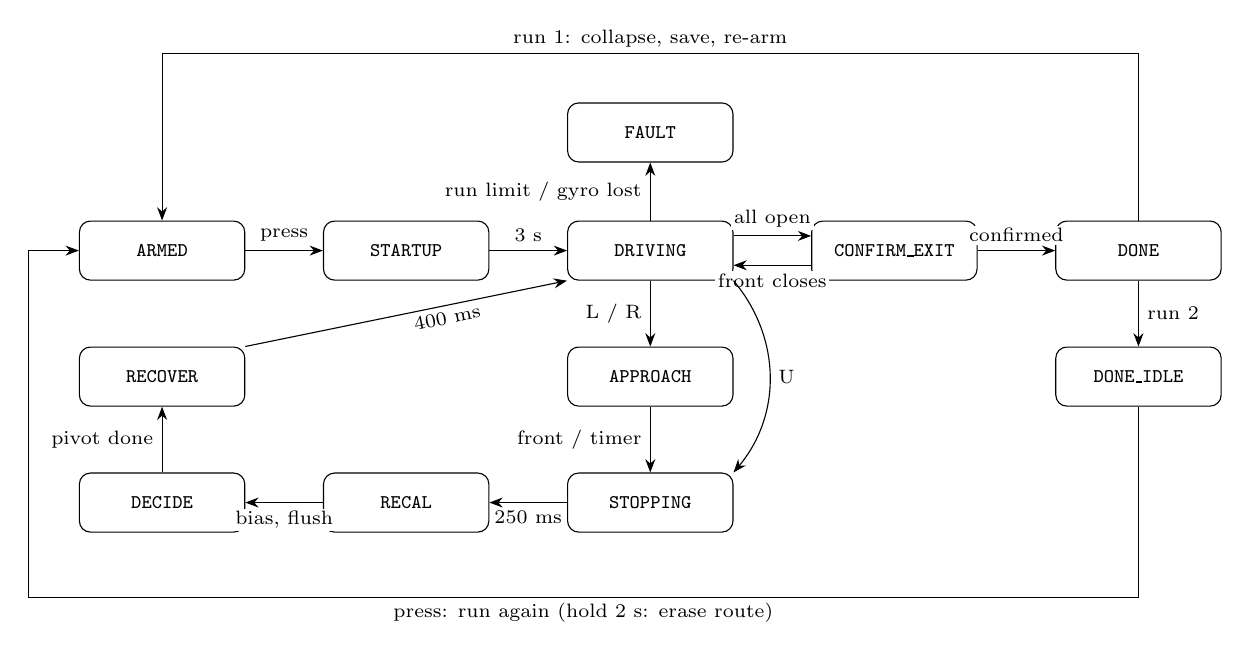
\begin{tikzpicture}[>=Stealth, font=\scriptsize,
    st/.style={rectangle, rounded corners, draw, minimum width=2.1cm,
               minimum height=0.75cm, font=\scriptsize\ttfamily, fill=white},
    lab/.style={font=\scriptsize, fill=white, inner sep=1pt}]
  % row 0
  \node[st] (armed) at (0,0)    {ARMED};
  \node[st] (start) at (3.1,0)  {STARTUP};
  \node[st] (drive) at (6.2,0)  {DRIVING};
  \node[st] (conf)  at (9.3,0)  {CONFIRM\_EXIT};
  \node[st] (done)  at (12.4,0) {DONE};
  % row 1
  \node[st] (rec)   at (0,-1.6)    {RECOVER};
  \node[st] (appr)  at (6.2,-1.6)  {APPROACH};
  \node[st] (idle)  at (12.4,-1.6) {DONE\_IDLE};
  % row 2
  \node[st] (dec)   at (0,-3.2)   {DECIDE};
  \node[st] (recal) at (3.1,-3.2) {RECAL};
  \node[st] (stop)  at (6.2,-3.2) {STOPPING};
  % fault
  \node[st] (fault) at (6.2,1.5)  {FAULT};

  \draw[->] (armed) -- node[lab, above=2pt] {press} (start);
  \draw[->] (start) -- node[lab, above=2pt] {3 s} (drive);
  \draw[->] (drive.10) -- node[lab, above=2pt] {all open} (conf.170);
  \draw[->] (conf.190) -- node[lab, below=2pt] {front closes} (drive.350);
  \draw[->] (conf) -- node[lab, above=2pt] {confirmed} (done);
  \draw[->] (drive) -- node[lab, left=2pt] {L / R} (appr);
  \draw[->] (appr) -- node[lab, left=2pt] {front / timer} (stop);
  \draw[->] (drive.south east) to[out=-50, in=50]
        node[lab, right=2pt] {U} (stop.north east);
  \draw[->] (stop) -- node[lab, below=2pt] {250 ms} (recal);
  \draw[->] (recal) -- node[lab, below=2pt] {bias, flush} (dec);
  \draw[->] (dec) -- node[lab, left=2pt] {pivot done} (rec);
  \draw[->] (rec.north east) -- node[lab, sloped, below=1pt, pos=0.62] {400 ms} (drive.south west);
  \draw[->] (drive) -- node[lab, left=2pt] {run limit / gyro lost} (fault);
  \draw[->] (done) -- node[lab, right=2pt] {run 2} (idle);
  \draw[->] (done.north) -- (12.4,2.5) -- node[lab, above=1pt] {run 1: collapse, save, re-arm} (0,2.5) -- (armed.north);
  \draw[->] (idle.south) -- (12.4,-4.4) -- node[lab, below=1pt] {press: run again (hold 2 s: erase route)} (-1.7,-4.4) -- (-1.7,0) -- (armed.west);
\end{tikzpicture}
\end{center}

\noindent
The run limit applies in DRIVING through RECOVER, and gyro loss in STARTUP
through RECOVER. Every one of those states can go to FAULT; only one such
edge is drawn.

\subsection{Sensor state machines}

\begin{itemize}
  \item \textbf{Opening debounce} is a saturating counter $c_t$:
        $c_{t+1} = \min(c_t+1, 255)$ if open, else 0; the side is declared
        open iff $c_t \ge 2$. A single bad ping can therefore never open a
        side.
  \item \textbf{Front vote} is a sliding window over the last 5 front
        distances; blocked iff $\ge 2$ are below the threshold. Unlike a
        consecutive-hit rule, a beam that swings on and off the target
        still accumulates votes.
  \item \textbf{Near-latch} is a counter bounded by 3, re-armed only by a
        real echo. The bound makes the latch provably self-terminating.
\end{itemize}

%% ==========================================================================
\section{Complexity analysis}\label{sec:complexity}
%% ==========================================================================

\subsection{Notation}

The maze is an $R\times C$ grid of cells, so $V = RC$. Adjacent cells are
joined by a passage when the wall between them is absent, so
\[
  |E| \le R(C-1) + C(R-1) = 2RC - R - C = \bigO{RC}.
\]
For a perfect maze $|E| = V-1$. Let $n$ be the number of log records
written in run 1, $n'$ the reduced length, and $W = 5$ the front vote
window.

\subsection{Exploration (run 1)}

\paragraph{Physical moves.} In a tree the left-hand walk is a prefix of an
Euler tour, in which every edge is traversed at most twice (once in each
direction):
\[
  \#\text{cell-to-cell moves} \;\le\; 2|E| \;=\; 2(V-1) \;=\; \bigO{RC}.
\]
Each move takes bounded physical time (at most one cell at
$\hat v \approx 40$\,cm/s, plus a bounded pivot), so the wall-clock time of
run 1 is $\bigO{RC}$.

\paragraph{Computation.} Each control tick does $\bigO{1}$ work: one ping,
one gyro read, a median of 3, a vote over $W$ entries, and constant-size
controller arithmetic. The per-tick cost is $\bigO{W} = \bigO{1}$ and
independent of the maze size.

\paragraph{Records.} One record per arrival at a decision cell. \code{s_passing}
prevents duplicates within one pass, so
\[
  n \;\le\; \sum_{v\ \text{decision}} \deg(v) \;\le\; 2|E| = \bigO{RC}.
\]
The hard cap \code{WALLMEM_MAX_RECORDS} $=48$ therefore limits the size of
maze that can be explored. Beyond it the run is flagged as unusable rather
than silently truncated.

\subsection{Collapse}

\paragraph{Current implementation.} Each outer iteration scans at most $n$
positions and, on a fold, calls \code{memmove} on at most $n$ bytes, then
restarts. Every fold reduces the length by 2, so there are
$f \le \lfloor n/2 \rfloor$ folds and $f+1$ outer iterations:
\[
  T_{\text{reduce}}(n) \;\le\; (f+1)\,(n + n) \;\le\;
  \left(\tfrac{n}{2}+1\right)\cdot 2n \;=\; n^2 + 2n \;=\; \bigO{n^2}.
\]
The bound is attained, up to constants, by logs whose U-turns all sit near
the end, because every rescan walks the whole folded prefix again. Space is
$\bigO{1}$ extra (in place). For $n \le 48$ this is at most about 2\,400
elementary steps, negligible at 16\,MHz, so the quadratic form is a
\emph{style} finding rather than a performance problem
(Finding~\ref{f:stack}).

\paragraph{Optimal alternative.} A single left-to-right pass with the output
prefix used as a stack gives $\bigO{n}$ time. Each record is pushed once;
each fold pops 3 and pushes 1, a net of $-2$, so at most $n/2$ folds occur
in total. By Lemma~\ref{lem:confluence} it produces the identical result.

\subsection{Replay (run 2)}

\code{WallMem_Play} is $\bigO{1}$ per junction (one index, one mask, one
compare), so $\bigO{n'}$ for the whole run. The physical time is
proportional to $|P(s,t)| \le V-1$.

\subsection{Persistence}

\code{WallMem_Save} writes $n+8$ bytes and reads $n+1$ back:
$\bigO{n}$ EEPROM operations (about 8.5\,ms per written byte on the ATmega32, so at most about 0.5\,s for 56 bytes, less when \code{eeprom_update_byte} skips unchanged cells; the robot is stopped). \code{WallMem_Load} reads
$n+6$ bytes and runs 8 CRC steps per byte: $\bigO{8n} = \bigO{n}$.

\subsection{Worst-case tick budget}

\begin{center}
\small
\begin{tabular}{@{}l r l@{}}
\toprule
Operation (per 20\,ms tick) & Bound & Reason \\
\midrule
Sonar ping & $\le 8.12$\,ms & two waits of \code{SONAR_TIMEOUT_US} $=4060$\,\textmu s \\
Gyro burst read, bus healthy & $\approx 0.85$\,ms & 9 bytes at 100\,kHz (90\,\textmu s per byte) plus start/stop \\
Gyro read, bus failing & $\lesssim 3$\,ms & one latched timeout ($\approx$1.4\,ms) plus recovery and re-wake \\
Supply ADC sample & $\approx 0.1$\,ms & 13 ADC clocks at 125\,kHz \\
Controller and solver logic & $\bigO{1}$ & fixed arithmetic, $W=5$ vote \\
\bottomrule
\end{tabular}
\end{center}
The sum stays below the 20\,ms period, with overruns counted if it ever does
not.

\subsection{Space}

\begin{center}
\small
\begin{tabular}{@{}l l l@{}}
\toprule
Structure & Size & Growth \\
\midrule
Junction log \code{s_log} & 48\,B & $\bigO{n}$, capped \\
Load staging \code{tmp} (stack, transient) & 48\,B & $\bigO{n}$ \\
EEPROM image & $8 + n \le 56$\,B & $\bigO{n}$ \\
Sonar state (3 sensors, 3-sample history) + vote window & $\approx 90$\,B & $\bigO{1}$ \\
Debug transmit ring & 192\,B & $\bigO{1}$ \\
Whole image, \code{.data}+\code{.bss} (avr-size) & 527\,B of 2\,048 & -- \\
\bottomrule
\end{tabular}
\end{center}
By contrast, a grid method would need $\Theta(RC)$ memory for walls and
distances. For example, a $16\times16$ flood fill needs at least $256$ bytes
of distances plus wall bits, which is half the SRAM this design uses in
total.

%% ==========================================================================
\section{Edge cases}
%% ==========================================================================

\subsection{Dead ends}
\begin{itemize}
  \item \textbf{Detection}: the front is blocked and both sides are closed
        for 3 consecutive ticks. A leg with no junction for 10\,s is also
        treated as a dead end, and goes through the \emph{same} logging path,
        so a wall the sonar never sees cannot desynchronise run 2.
  \item \textbf{Manoeuvre}: two 90\textdegree{} halves, rotating towards the
        roomier side, with a measured clearance creep at the halfway point
        and a second half that targets 180\textdegree{} in total.
  \item \textbf{Memory}: the $U$ record is always folded away by the
        collapse, so run 2 never enters a dead end.
\end{itemize}

\subsection{Cyclic paths (loops)}\label{sec:cycles}
\begin{itemize}
  \item \textbf{Termination}: the left-hand rule reaches the exit if the
        start is on the same wall component as the exit (for instance, both
        on the outer boundary). If the robot starts beside an \emph{island}
        (a wall component not connected to the boundary), it circles
        forever. The code bounds this with \code{MAX_RUN_MS} (5\,min)
        $\to$ \code{WM_FAULT}.
  \item \textbf{Reduction}: a loop traversed by the wall follower produces
        no U-turn, so nothing folds it away. The replayed route is still a
        valid walk to the exit, but it is not necessarily the shortest.
  \item \textbf{Stray-U check}: the code treats a surviving U as ``maze has
        a loop or a junction was misread''. That implication holds one way
        only. A stray U means the log is not a tree traversal, but zero
        stray U's does \emph{not} prove the maze is loop-free or that the
        route is shortest (Finding~\ref{f:loop}). There is no visited set,
        and without localisation there cannot be one, so loops cannot be
        detected in general.
\end{itemize}

\subsection{Disconnected paths and an unreachable exit}
There is no map, so unreachability cannot be proved. The robot follows its
wall component until the run limit ends the attempt with a fault, and the
log is not saved (it never reaches \code{WM_DONE}). This is the correct
fail-safe for a design without localisation.

\subsection{Out-of-bounds and overflow checks}
There are no grid coordinates to overflow. The analogous checks are array
and integer bounds:

\begin{center}
\small
\begin{tabularx}{\linewidth}{@{}l X@{}}
\toprule
Site & Guard \\
\midrule
\code{WallMem_Record} & \code{s_count >= 48} $\Rightarrow$ drop, set overflow, run not saved \\
\code{WallMem_Reduce} scan & $1 \le i$ and $i+1 < n$: both neighbours exist; \code{memmove} length $n-(i+2) \ge 0$ \\
\code{WallMem_At} & returns \code{0xFF} (an invalid record) for $i \ge n$ \\
\code{WallMem_Play} & \code{EXHAUSTED} when the cursor reaches $n$ \\
\code{WallMem_Load} & $n>48$, a bad zero-bit mask or a CRC mismatch $\Rightarrow$ reject \\
Sonar rings & indices advanced modulo \code{HIST} / \code{FRONT_VOTE_WINDOW} / \code{SONAR_COUNT} \\
Debounce counters & saturate at 255 rather than wrapping to 0 \\
\code{millis()} wrap (49.7 days) & all comparisons use unsigned differences \\
Heading accumulator & \code{int32}; \code{Heading_DegreesTenths} multiplies by 10, so it overflows beyond $|\Theta| \approx 2^{31}/10/64711 \approx 3\,300^\circ$. Safe, because the accumulator is reset at every stop and pivot; only the armed spin-calibration printout could approach it, after about 9 full hand turns \\
Gyro clipping & $\pm500$\,\textdegree/s range; \code{peak_rate} is reported so a clipped (under-integrated) turn is visible \\
\bottomrule
\end{tabularx}
\end{center}

\subsection{Maze boundary and exit}
The exit is recognised by all three sides opening, then confirmed by driving
\code{EXIT_CONFIRM_CM} (25\,cm) without the front closing. A four-way
junction seen early would otherwise look identical. The compile-time
\code{\#error} in \file{config.h} enforces that the window exceeds two
debounce periods of travel.

\subsection{Sensing edge cases}
\begin{itemize}
  \item \textbf{No echo vs.\ too close}: kept distinct. A too-close wall is
        never reported as open.
  \item \textbf{Busy sensor}: never timed; treated as no echo.
  \item \textbf{Unmeasured side after a flush}: never counted
        (\code{Sonar_HasSample}).
  \item \textbf{Junction's own far wall}: forward is not declared open while
        the front wall is within 50\,cm and a side is open.
  \item \textbf{Opening right after a pivot}: the approach is timed from
        the pivot cell, because no leading edge was seen.
\end{itemize}

\subsection{Replay divergence and hardware faults}
\begin{itemize}
  \item \textbf{Mismatch / exhausted}: degrade to the left-hand rule (or
        halt, if configured). The run still finishes on a loop-free maze.
  \item \textbf{Gyro bus}: bounded waits, bus recovery, and a stop after
        100\,ms of loss.
  \item \textbf{Freeze}: the 250\,ms watchdog, with motors stopped first on
        reboot.
  \item \textbf{Power loss during save}: the magic byte is written last, so
        a partial block is rejected.
\end{itemize}

%% ==========================================================================
\section{Findings and optimisations}
%% ==========================================================================

Ordered by expected impact on the robot. \emph{Algorithmic} findings do not
change behaviour on a correctly classified perfect maze. \emph{Robustness}
findings do.

\begin{finding}[Robustness: heading is never held]\label{f:dead}
\code{drive.c} declares \code{s_hold_heading} and never reads it.
\code{turn_result_t.residual_raw} (\file{turn.h}) documents a hand-off to
\code{Drive_StraightHold()}, a function that does not exist. After a pivot
that lands a few degrees off, the only corrective signal is the lateral
wall error, which appears only after the robot has drifted. The gyro term
is pure rate damping and even resists the needed correction.
\emph{Recommendation}: a cascaded controller in which the wall error sets a
small heading target, the heading error sets a desired yaw rate, and the gyro
closes the rate loop. Seed it with \code{residual_raw} after every turn.
Remove the dead variable and the stale comment either way.
\end{finding}

\begin{finding}[Robustness: distance is inferred from time]
\code{APPROACH_TIME_MS}, \code{POST_TURN_CELL_MS} and \code{EXIT_CONFIRM_MS}
all divide a distance by \code{TRAVEL_SPEED_CMS}. The logs show that speed
ranging over 34--43\,cm/s with battery charge and steering load. Wheel
encoders would remove this error source entirely, and would also make a
localised algorithm (flood fill) possible. Without encoders, re-measuring
the constant per battery is the mitigation.
\end{finding}

\begin{finding}[Algorithmic: loops are not detectable]\label{f:loop}
``No stray U'' is necessary but not sufficient for ``the route is the
shortest path''. On a maze with cycles the replay remains valid (it is the
successful run-1 walk without its dead ends) but may be longer than
optimal. The comment at \file{solver.c:647} overstates the guarantee.
\emph{Recommendation}: document the requirement that the maze be
loop-free, as \code{WM_DONE}'s message already partly does.
\end{finding}

\begin{finding}[Algorithmic: a leading U is reported as a failure]
A U-turn at index 0 (the robot starts facing a dead end) has no left
neighbour, so it survives the collapse and marks the run unsaveable, even
though it is a legitimate first move that replays correctly (its signature
matches). \emph{Fix}: exclude index 0 from the stray count, i.e.\ start the
counting loop at \code{i = 1}.
\end{finding}

\begin{finding}[Complexity: collapse is quadratic]\label{f:stack}
The rescan after every fold gives $\bigO{n^2}$. A stack pass is $\bigO{n}$,
in place, and needs no \code{memmove}:

\begin{lstlisting}[numbers=none]
uint8_t WallMem_Reduce(uint8_t *stray_u_out) {
    uint8_t rd, top = 0, stray = 0;           /* s_log[0..top) is the stack */
    for (rd = 0; rd < s_count; rd++) {
        s_log[top++] = s_log[rd];              /* push                      */
        while (top >= 3 && WallMem_Turn(s_log[top - 2]) == WM_TURN_U) {
            uint8_t b = WallMem_Turn(s_log[top - 1]);
            uint8_t a = WallMem_Turn(s_log[top - 3]);
            s_log[top - 3] = (uint8_t)(WallMem_Sig(s_log[top - 3]) |
                                       ((a + b + 2u) & WM_TURN_MASK));
            top -= 2;                          /* pop U and B, keep folded A */
        }
    }
    s_count = top;
    for (rd = 0; rd < s_count; rd++)
        if (WallMem_Turn(s_log[rd]) == WM_TURN_U) stray++;
    if (stray_u_out) *stray_u_out = stray;
    if (stray == 0) s_solved = 1;
    s_play_index = 0;
    return s_count;
}
\end{lstlisting}
The \code{while} loop handles cascades ($L\,U\,R \mapsto U$ folding again
with its own neighbours). Equivalence with the current version follows from
Lemma~\ref{lem:confluence}. The existing host test \file{test/test_wallmem.c}
(fold table, nested dead end, storage, corruption) covers exactly the
properties to re-check after the change.
\end{finding}

\begin{finding}[Memory: fold online during run 1]
Applying the same stack step inside \code{WallMem_Record} keeps the log
reduced at all times. Its length is then bounded by the depth of the current
start-to-junction path instead of the total number of decision visits, so a
maze that needs more than 48 raw records but fewer than 48 path records
becomes solvable with no RAM increase. The collapse at \code{WM_DONE}
becomes a no-op.
\end{finding}

\begin{finding}[Runtime: blocking sonar]
\code{ping()} busy-waits for up to 8.1\,ms of every 20\,ms tick. Timing
the echo with pin-change interrupts on PORTA, or with the input-capture
unit, would make ranging non-blocking and remove most of the tick jitter
that the gyro integration depends on.
\end{finding}

\begin{finding}[Minor]
\begin{itemize}
  \item \code{WallMem_Load} stages records in a 48-byte stack array. It
        could validate in place against \code{s_log} with a single rollback
        flag, saving 48\,B of peak stack. This is low priority at 527\,B of
        2\,KB used.
  \item The record uses 5 of its 8 bits. Packing is not worthwhile: the
        zero bits are the corruption check.
  \item CRC-8 does not cover the two magic bytes, but they are compared
        literally, so nothing is lost.
\end{itemize}
\end{finding}

%% ==========================================================================
\appendix
\section{Key constants (\textsf{config.h})}
%% ==========================================================================

\begin{center}
\small
\begin{longtable}{@{}l r l@{}}
\toprule
Constant & Value & Meaning \\
\midrule
\endhead
\code{CONTROL_TICK_MS} / \code{TURN_TICK_MS} & 20 / 5\,ms & main loop / pivot loop period \\
\code{CORRIDOR_WIDTH_CM} & 40\,cm & cell size \\
\code{SONAR_TO_AXLE_CM} & 15\,cm & sensor ahead of the pivot axis \\
\code{TRAVEL_SPEED_CMS} & 40\,cm/s & measured 34--43 \\
\code{APPROACH_TIME_MS} & 875\,ms & $(15+20)/40$\,s \\
\code{POST_TURN_CELL_MS} & 1000\,ms & $40/40$\,s \\
\code{EXIT_CONFIRM_CM} / \code{_MS} & 25\,cm / 625\,ms & exit confirmation window \\
\code{OPENING_THRESHOLD_CM} & 30\,cm & side counts as open beyond this \\
\code{FRONT_BLOCKED_CM} / \code{FRONT_STOP_CM} & 25 / 12\,cm & front classification / approach stop \\
\code{JUNCTION_FRONT_WALL_CM} & 50\,cm & ``the junction's own far wall'' \\
\code{OPENING_CONFIRM} / \code{DEADEND_CONFIRM} & 2 / 3 ticks & debounce depths \\
\code{FRONT_VOTE_WINDOW} / \code{_THRESHOLD} & 5 / 2 & front vote \\
\code{SONAR_MAX_RANGE_CM} / \code{MIN_VALID} & 70 / 3\,cm & ranging limits \\
\code{DRIVE_BASE_PWM} & 60 & cruise \\
\code{MOTOR_MIN_PWM} / \code{MAX} & 45 / 140 & PWM clamp \\
\code{WALL_KP} / \code{WALL_KD} & 3/2 / 1/65 & centring gains \\
\code{WALL_MAX_CORRECTION_RATIO_PCT} & 37\,\% & $|u|\le 22$ at base 60 \\
\code{TURN_PWM} / \code{TURN_STOP_MARGIN_DEG} & 85 / 28\textdegree & sweep speed / early cut \\
\code{TURN_DEADBAND_DEG} / \code{TURN_MAX_NUDGES} & 2\textdegree{} / 8 & pivot acceptance \\
\code{GYRO_LSB_MS_PER_DEGREE} & 64\,711 & hand-calibrated scale \\
\code{GYRO_FAIL_MS} / \code{I2C_TIMEOUT_US} & 100\,ms / 1\,ms & gyro-loss detection \\
\code{MAX_LEG_MS} / \code{MAX_RUN_MS} & 10\,s / 5\,min & safety limits \\
\code{WALLMEM_MAX_RECORDS} & 48 & log capacity \\
\bottomrule
\end{longtable}
\end{center}

\end{document}
